\chapter{Réalisation}


\section{Introduction}
Cette partie constitue le dernier volet de ce rapport. Après avoir terminé la phase de l'analyse et la conception, nous présentons les outils et l’environnement logiciel de développement utilisés ainsi que les différents captures du projet.\\
\section{Outils et technologies}
\subsection{Langage de programmation}
Java Platform, Enterprise Edition ou Java EE, est une spécification pour la plate-forme Java d'Oracle, destinée aux applications d'entreprise.
La plate-forme étend Java Platform, Standard Edition (Java SE) en fournissant une API de mapping objet-relationnel, des architectures distribuées et multitiers, et des services web3. La plate-forme se fonde principalement sur des composants modulaires exécutés sur un serveur d'applications.\\
\begin{figure}[!h]
\begin{center}

\includegraphics[height=3cm]{Pictures/jee.png}
\end{center}
\caption{Logo Java EE}
\end{figure}

\\ \par 
GlassFish est un projet de serveur d'applications de plateforme open source Jakarta EE lancé par Sun Microsystems, alors sponsorisé par Oracle Corporation, et résidant désormais à la Fondation Eclipse et soutenu par Payara, Oracle et Red Hat. La version prise en charge sous Oracle s'appelait Oracle GlassFish Server
\\
\begin{figure}[!h]
\begin{center}

\includegraphics[height=4cm]{Pictures/glassfish.png}
\end{center}
\caption{Logo Glassfish}
\end{figure}

\\ \par 
HTML est un langage dit de « marquage », de « structuration » ou de « balisage » dont le rôle est de formaliser l’écriture d’un document avec des balises de formatage. Les balises permettent d’indiquer la façon dont doit être présenté le document et les liens qu’il établit avec d’autres documents.
\\
\begin{figure}[!h]
\begin{center}

\includegraphics[height=3cm]{Pictures/HTML.png}
\end{center}
\caption{Logo HTML}
\end{figure}

\\ \par 
Les feuilles de style en cascade, généralement appelées CSS de l'anglais Cascading Style Sheets, forment un langage informatique qui décrit la présentation des documents HTML et XML. Les standards définissant CSS sont publiés par le World Wide Web Consortium (W3C). Introduit au milieu des années 1990, CSS devient couramment utilisé dans la conception de sites web et bien pris en charge par les navigateurs web dans les années.
\\
\begin{figure}[!h]
\begin{center}

\includegraphics[height=3cm]{Pictures/css.png}
\end{center}
\caption{Logo CSS}
\end{figure}

\\ \par 
JavaScript est un langage de programmation qui permet d’implémenter des mécanismes complexes sur une page web. À chaque fois qu’une page web fait plus que simplement afficher du contenu statique — afficher du contenu mis à jour à des temps déterminés, des cartes interactives, des animations 2D/3D, des menus vidéo défilants, etc... — JavaScript a de bonnes chances d’être impliqué. C’est la troisième couche des technologies standards du web, les deux premières (HTML et CSS).
\\
\begin{figure}[!h]
\begin{center}

\includegraphics[height=3cm]{Pictures/js.png}
\end{center}
\caption{Logo JavaScript}
\end{figure}


%\cite{cite2} 
%---------------Environnement de développement------------------
\subsection{Environnement de développement}
Docker est un ensemble de produits de plate-forme en tant que service (PaaS) qui utilisent la virtualisation au niveau du système d'exploitation pour fournir des logiciels dans des packages appelés conteneurs. Les conteneurs sont isolés les uns des autres et regroupent leurs propres logiciels, bibliothèques et fichiers de configuration; ils peuvent communiquer entre eux via des canaux bien définis. Étant donné que tous les conteneurs partagent les services d'un seul noyau de système d'exploitation, ils utilisent moins de ressources que les machines virtuelles.
\\
\begin{figure}[!h]
\begin{center}

\includegraphics[height=3.5cm]{Pictures/docker.png}
\end{center}
\caption{Logo Docker}
\end{figure}
\newline
\\ \par 
Maven est un puissant outil de gestion de projet basé sur POM (Project Object Model). Il est utilisé pour la construction de projets, les dépendances et la documentation. Cela simplifie le processus de construction comme ANT. Mais c'est trop avancé que ANT.\newline
En bref, nous pouvons dire que maven est un outil qui peut être utilisé pour créer et gérer n'importe quel projet basé sur Java. maven facilite le travail quotidien des développeurs Java et aide généralement à la compréhension de tout projet basé sur Java.
\\
\begin{figure}[!h]
\begin{center}
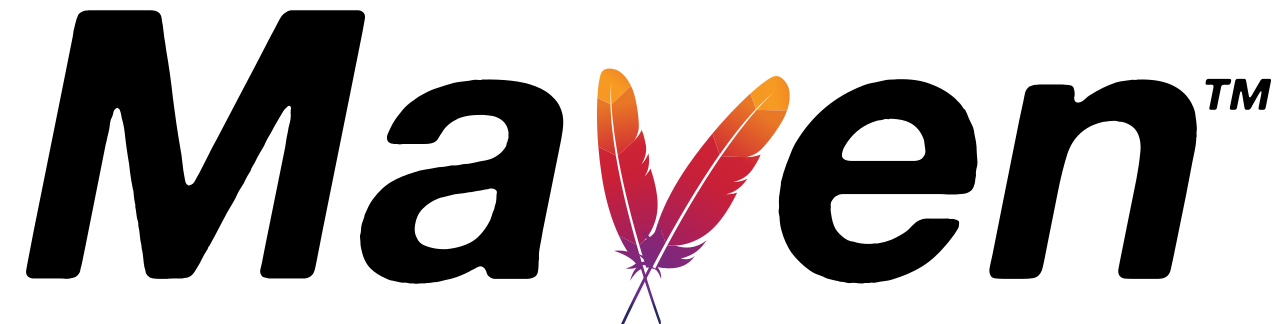
\includegraphics[height=2.5cm]{Pictures/maven.png}
\end{center}
\caption{Logo Maven}
\end{figure}

\subsection{Gestion de version et de collaboration}
Git est un logiciel de gestion de versions décentralisé. C'est un logiciel libre créé par Linus Torvald, auteur du noyau Linux, et distribué selon les termes de la licence publique générale GNU version 2. En 2016, il s'agit du logiciel de gestion de versions le plus populaire qui est utilisé par plus de douze millions de personnes.
\\
\begin{figure}[!h]
\begin{center}

\includegraphics[height=3cm]{figures/git.png}
\end{center}
\caption{Git}
\end{figure}



%---------------Communication------------------
\subsection{Outils de Communication}
Google Meet est un service de video conférence developpé par Google. Il est utilisé au sein de l'entreprise Daba'Go pour effectué des réunions avec des partenaires aussi bien une réunion pour tous les collaborateurs, elle est toujours programmée chaque vendredi après-midi pour se rencontrer tous et discuter les avancements dans chaque équipe.
\\
\begin{figure}[!h]
\begin{center}

\includegraphics[height=1cm]{figures/google_meet_logo.png}
\end{center}
\caption{Google Meet}
\end{figure}

\newpage
\section{Intérfaces}


\begin{figure}[htb!]
  \centering

\includegraphics[height=0.43\paperwidth,width=0.8\paperwidth]{Pictures/Home.png}
\caption{Page Home}
\end{figure}
\FloatBarrier

\begin{figure}[htb!]
  \centering
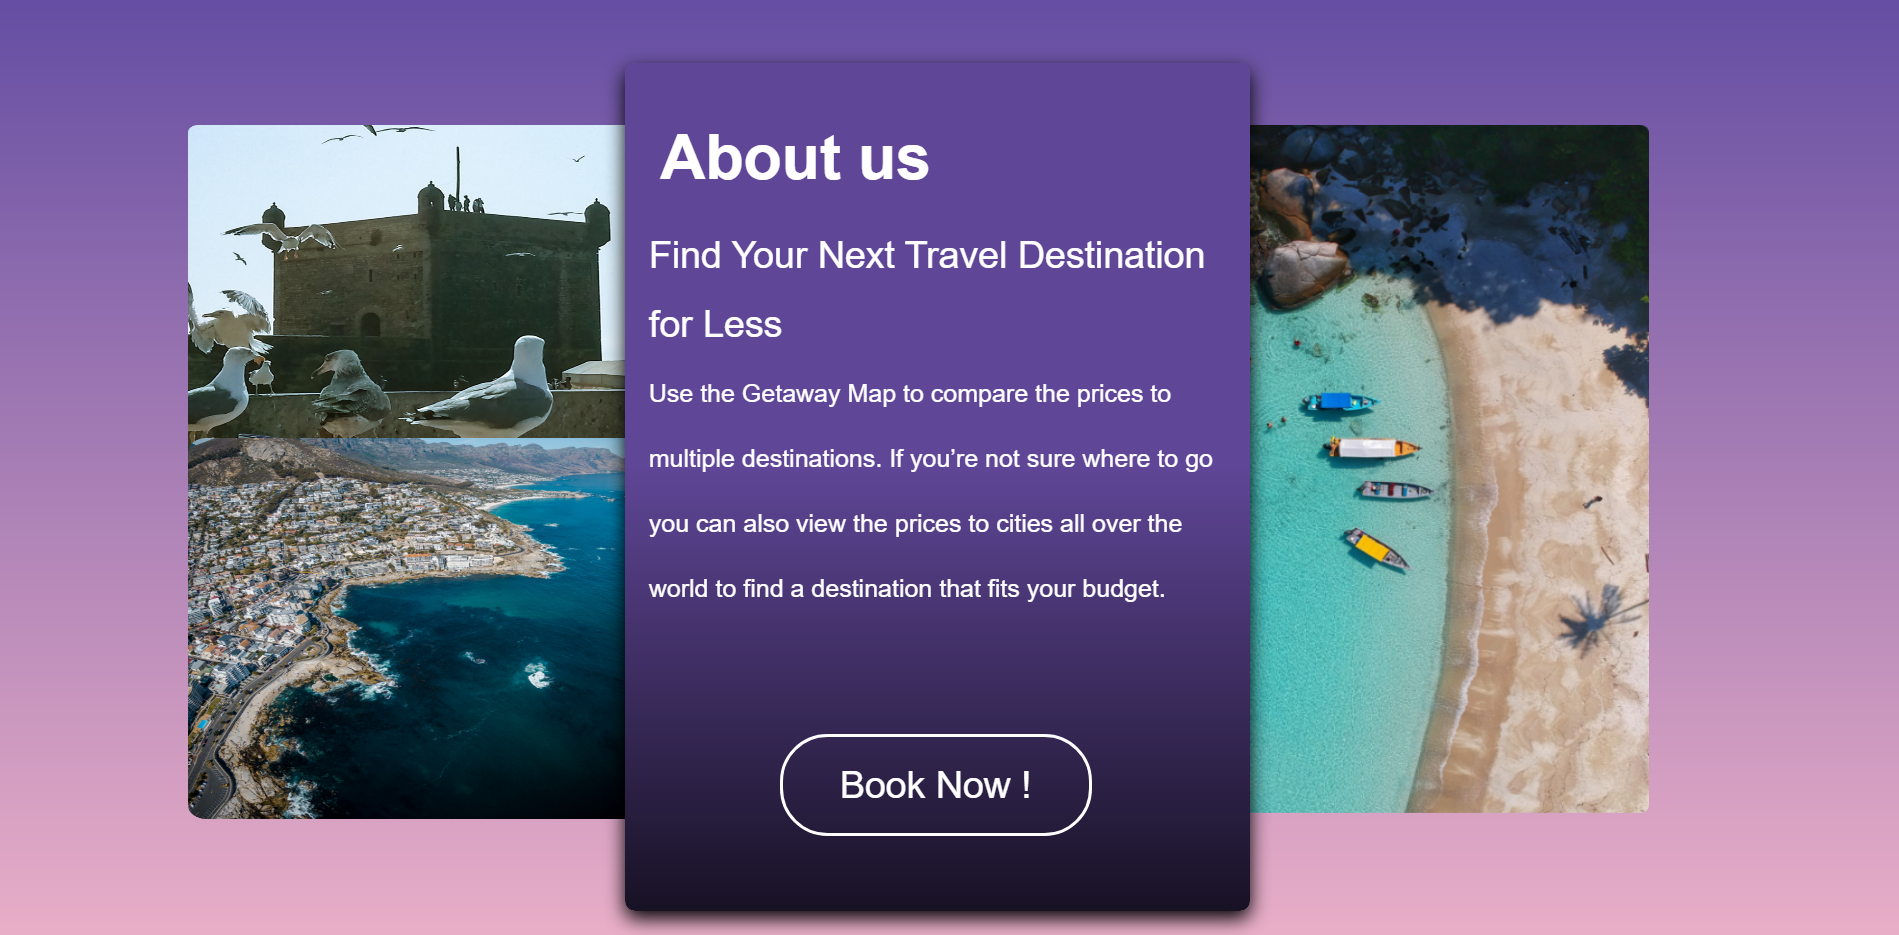
\includegraphics[height=0.43\paperwidth,width=0.8\paperwidth]{Pictures/About us.png}
\caption{About us}
\end{figure}
\FloatBarrier



\begin{figure}[htb!]
  \centering
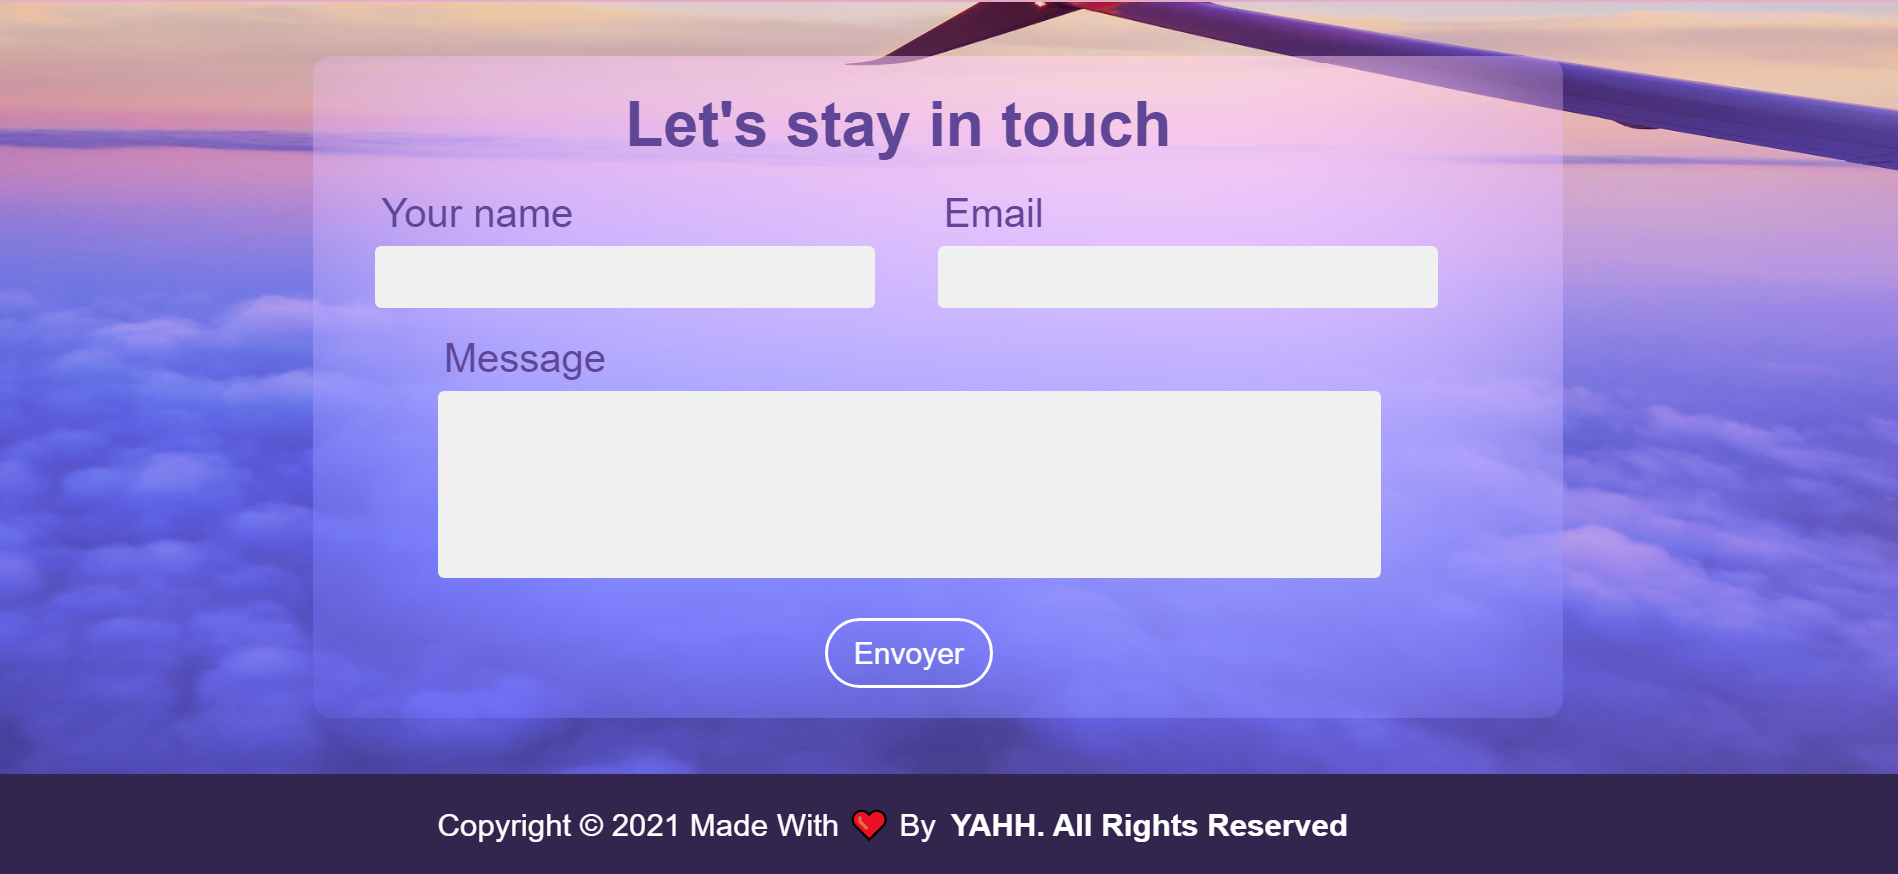
\includegraphics[height=0.43\paperwidth,width=0.8\paperwidth]{Pictures/Contact us.png}
\caption{Contact Us}
\end{figure}
\FloatBarrier


\begin{figure}[htb!]
  \centering
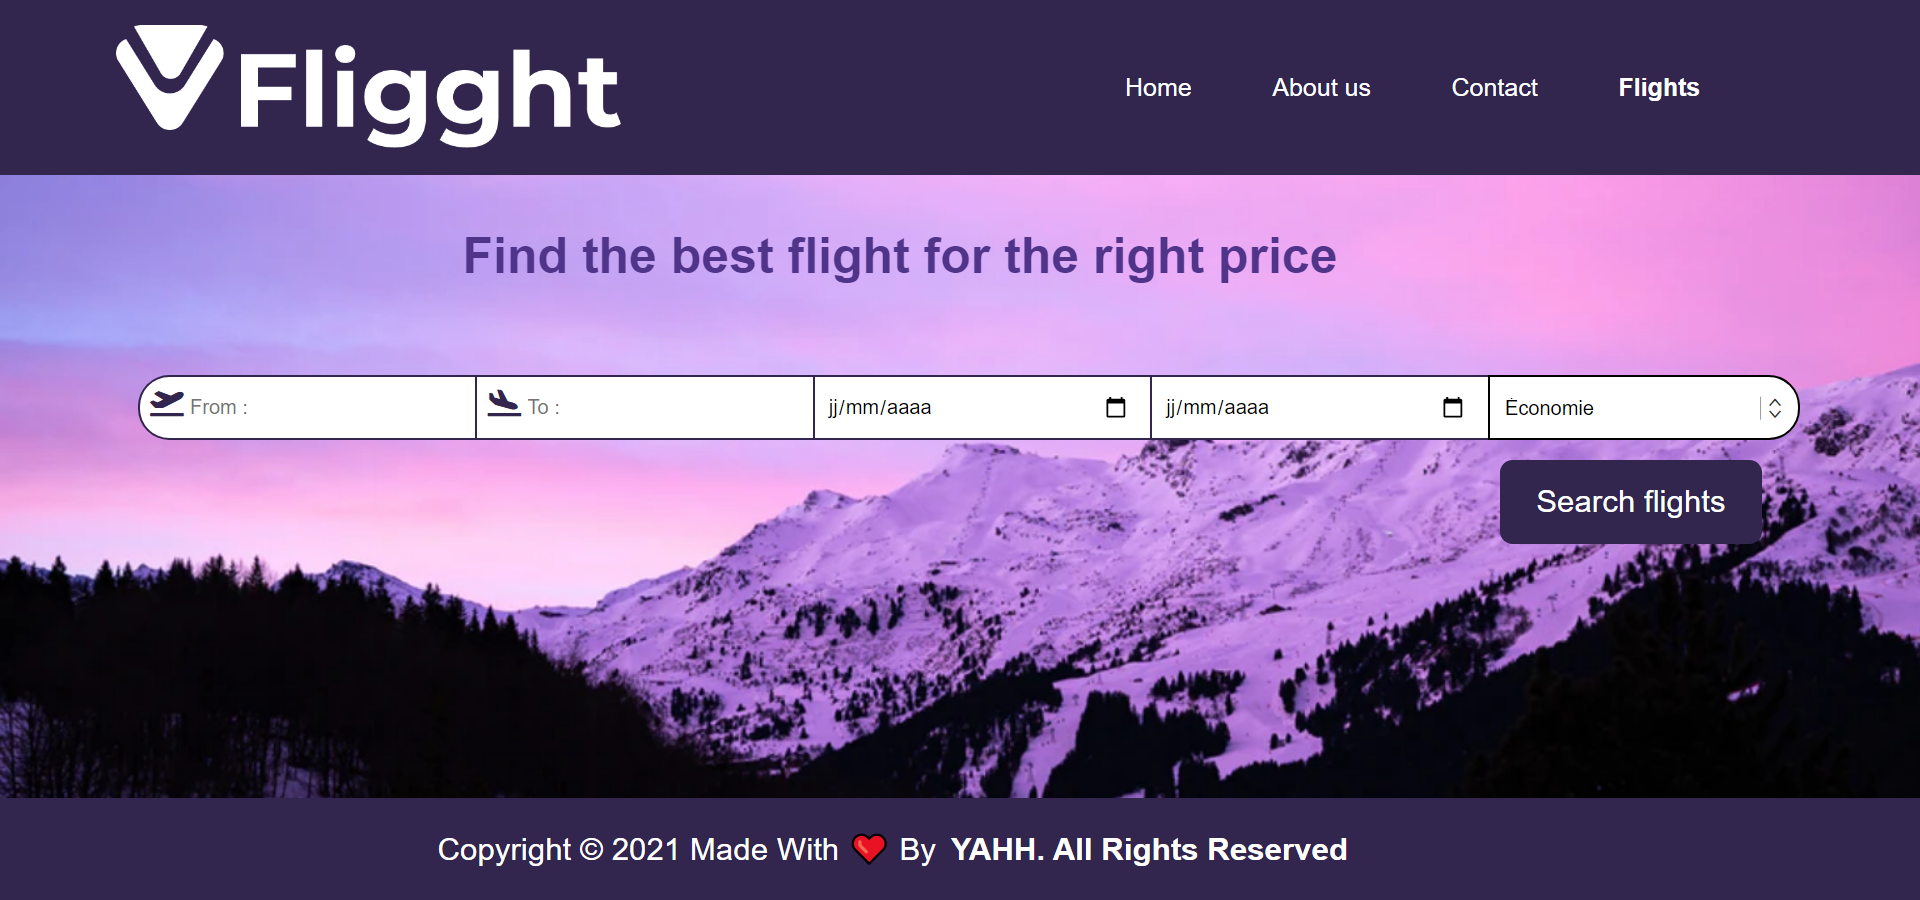
\includegraphics[height=0.43\paperwidth,width=0.8\paperwidth]{Pictures/Search.png}
\caption{Search for flights}
\end{figure}
\FloatBarrier

\begin{figure}[htb!]
  \centering
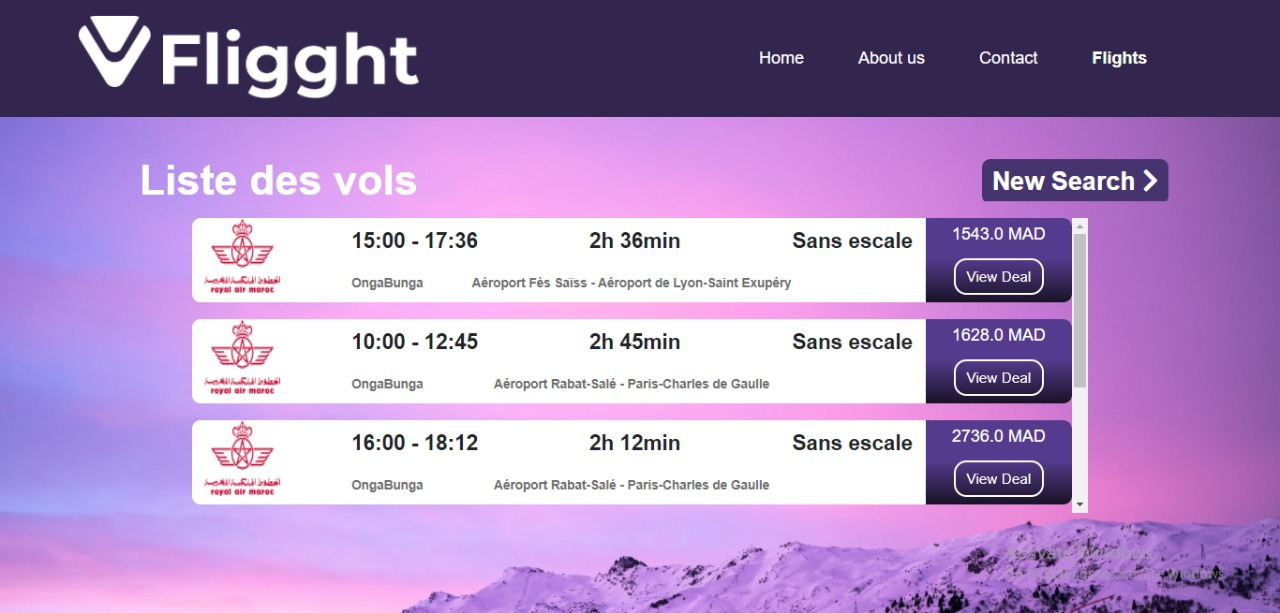
\includegraphics[height=0.43\paperwidth,width=0.8\paperwidth]{Pictures/Result.jpeg}
\caption{Search result}
\end{figure}
\FloatBarrier
